\documentclass[10pt]{beamer}

\usetheme{metropolis}
\usepackage{appendixnumberbeamer}

\usepackage{outlines}

\title{Extending Distributed Functionality in Phylanx}
\subtitle{Master's Defense}
\author{Maxwell Reeser}
\date{March 24, 2020}
\institute{Division of Computer Science and Engineering \\ School of Electrical Engineering and Computer Science \\ Louisiana State University}
\titlegraphic{
\includegraphics[height=10mm]{logos/stellar_4x1.pdf}}
\titlegraphic{
	\begin{tikzpicture}[overlay, remember picture]
	\node[at=(current page.south east), anchor=south east] {%
		
\includegraphics[width=.25\textwidth]{logos/stellar_4x1.pdf} 
	};
	\node[at=(current page.south west), anchor=south west] {%
		
\includegraphics[width=.50\textwidth]{logos/cct_logo.pdf} 
	};
	\end{tikzpicture}
}


\begin{document}
\setbeamercolor{background canvas}{bg=white}
\maketitle

\begin{frame}{Previous Publications/Presentations}
	\begin{outline}
		\1 This presentation was delivered at the SCALA 2020 conference
	\end{outline}
\end{frame}

%\begin{frame}{Outline}
%  \setbeamertemplate{section in toc}[sections]
%  \tableofcontents[hideallsubsections]
%\end{frame}
\begin{frame}{Outline}
	\setbeamertemplate{section in toc}[sections]
	\tableofcontents[hideallsubsections]
\end{frame}

\section{Introduction to Phylanx and Background}

\begin{frame}{Phylanx: An Asynchronous Distributed C++ Array Processing Toolkit}
	\begin{outline}
		\1 Write Python code, run it in distributed
		\1 Targeting machine learning mainly
			\2 Focus on linear algebra
			\2 Lower barrier to entry for ML Practitioners
				\3 NumPy API 
		\1 Heavy use of HPX			
			\2 Standard's compliant distributed C++ runtime
			\2 Product of Stellar Group
		\1 Blaze data structures
			\2 Parallel linear algebra
	\end{outline}
\end{frame}

\begin{frame}{Distributed Phylanx Roadmap}
	\begin{outline}
		\1 Map operations 
		\2 No Data Dependencies
		\1 Distributed Data Structures
		\2 distributed\_object
		\3 UPC++
		\2 distributed\_vector/matrix
		\2 Annotations
		\1 Distributed Primitives
			\2 Previously implemented:
				\3 Matrix transpose
				\3 Vector-vector product
				\3 Matrix-vector product
			\2 Implemented in this project:
				\3 Matrix-matrix product
	\end{outline}
\end{frame}

\begin{frame}{Tiling in Phylanx}
	\begin{outline}
		\1 Distributed computation means distributed data
		\2 Distributed data structures have local (single node) tiles
		\2 These can be tiles of vectors, matrices, or other data structures
		\2 Splitting up of data must be intentional
		\2 We mostly focus on tiling of matrices
		\1 Different tilings can have different costs
		\2 Eventually we want to minimize the cost
	\end{outline}
\end{frame}

\begin{frame}{Tiling Example: $A = B + C$}
	\begin{figure}	
		\centering
		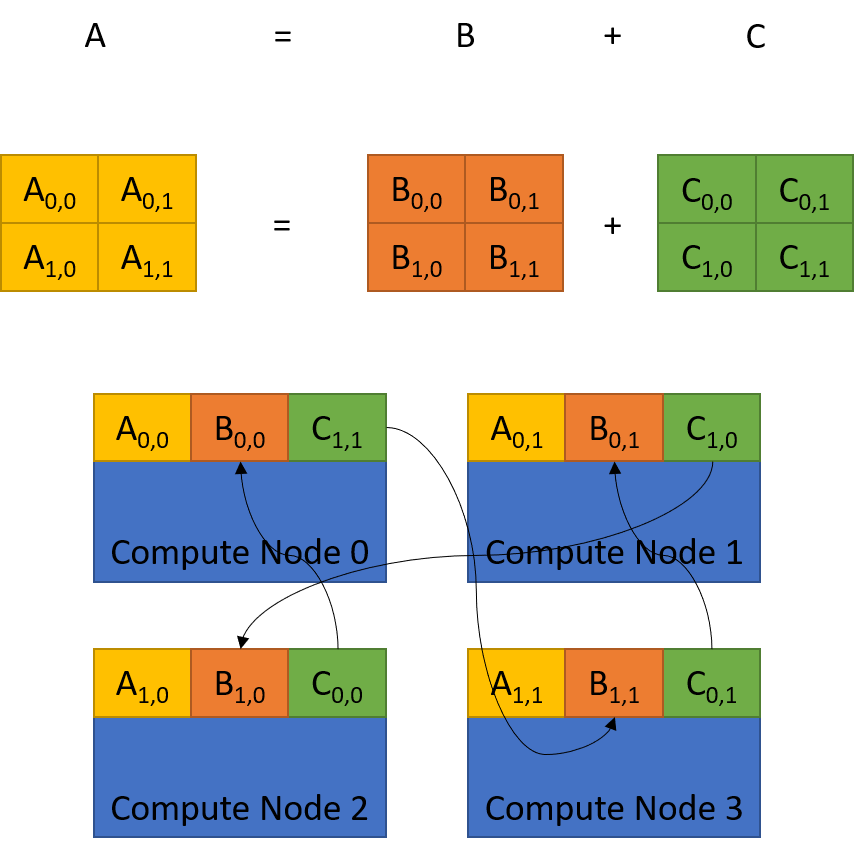
\includegraphics[width=0.66\linewidth]{figures/network_communication_fix_misalignment.png}
		\caption{Tiling Mismatch}
	\end{figure}
\end{frame}


\begin{frame}{distributed\_matrix}
	\begin{outline}
		\1 Object-oriented distributed data organization
		\1 Enabled by HPX's Active Global Address Space (AGAS)
		\1 Maintains a list of participating nodes
		\1 Allows one local tile to "fetch" a non-local tile over the network			
	\end{outline}
\end{frame}

\begin{frame}{distributed\_matrix Example}
	\begin{figure}	
		\centering
		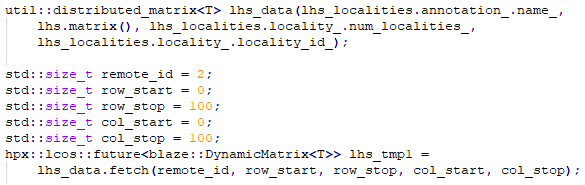
\includegraphics[width=0.85\linewidth]{figures/dist_matrix_lhs.png}
		\caption{Tiling Mismatch}
	\end{figure}
\end{frame}

\section{Algorithms}

\begin{frame}{dot\_d 2d2d \& Cannon Product}
	\begin{outline}
		\1 dot\_d 2d2d
			\2 Supports rectangular, non-overlapping tiling on an arbitrary number of nodes
			\2 Designed by Hartmut Kaiser
		\1 Cannon Product
			\2 Requires uniform tiling on a perfect square number of nodes
			\2 Chosen for its simplicity and space efficiency
	\end{outline}
\end{frame}

\begin{frame}{dot\_d 2d2d}
\begin{outline}
	\1 Very flexible matrix multiplication algorithm
	\1 Iterates through all tiles of RHS operand
		\2 Performs multiplication if intersection detected
	\1 Local partial result matrices may be large
	\1 May require partial result row-aggregation in order to compute final result
\end{outline}
\end{frame}

\begin{frame}{dot\_d Example: $A = B \cdot C$}
	\begin{figure}	
		\centering
		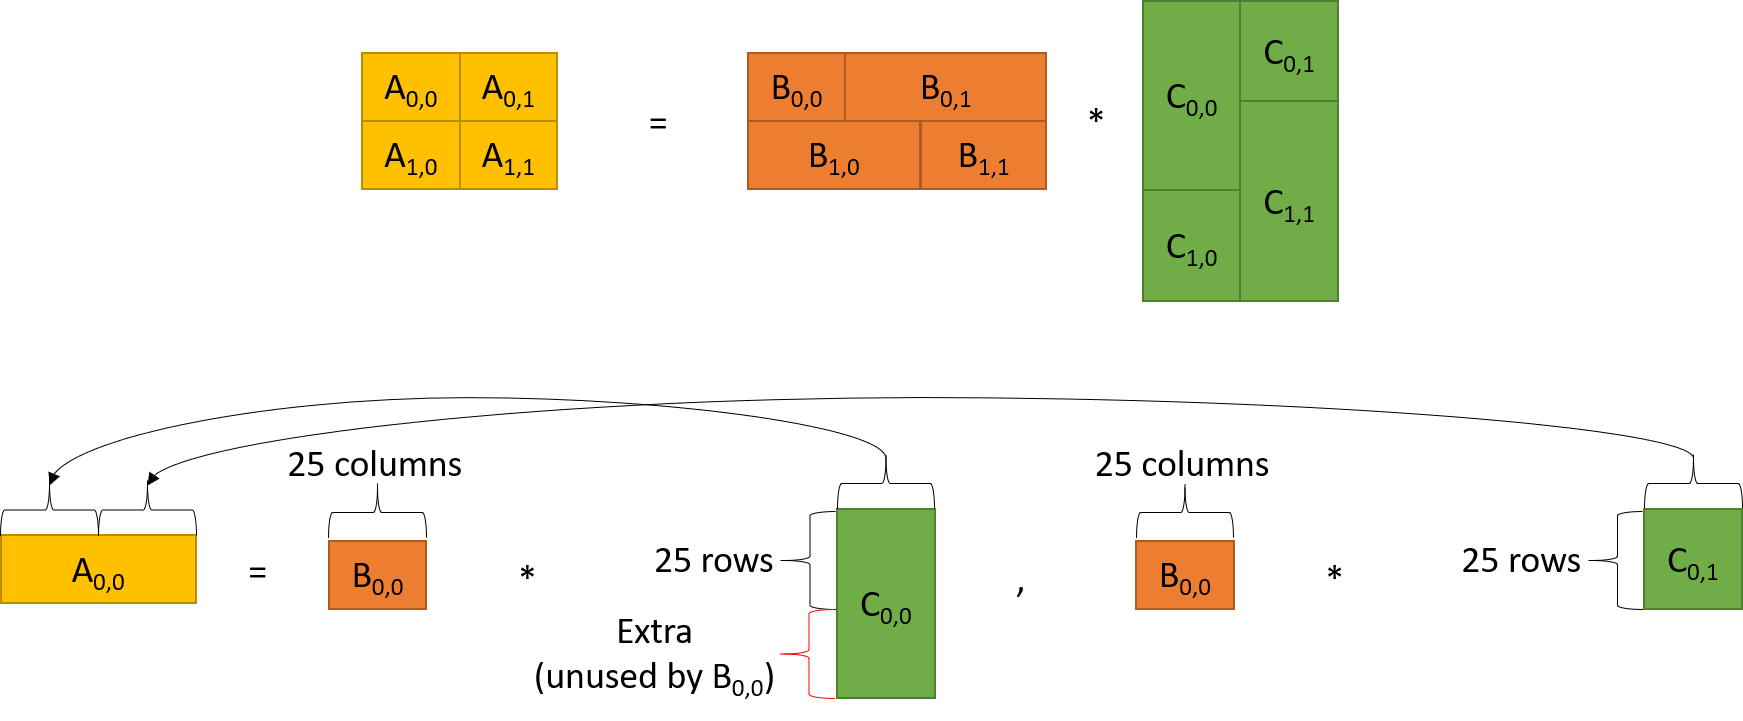
\includegraphics[width=0.72\linewidth]{figures/intermediate_result.png}
		\caption{Calculating Intermediate Result}
	\end{figure}
\end{frame}

\begin{frame}{dot\_d Example: $A = B \cdot C$ }
	\begin{figure}	
		\centering
		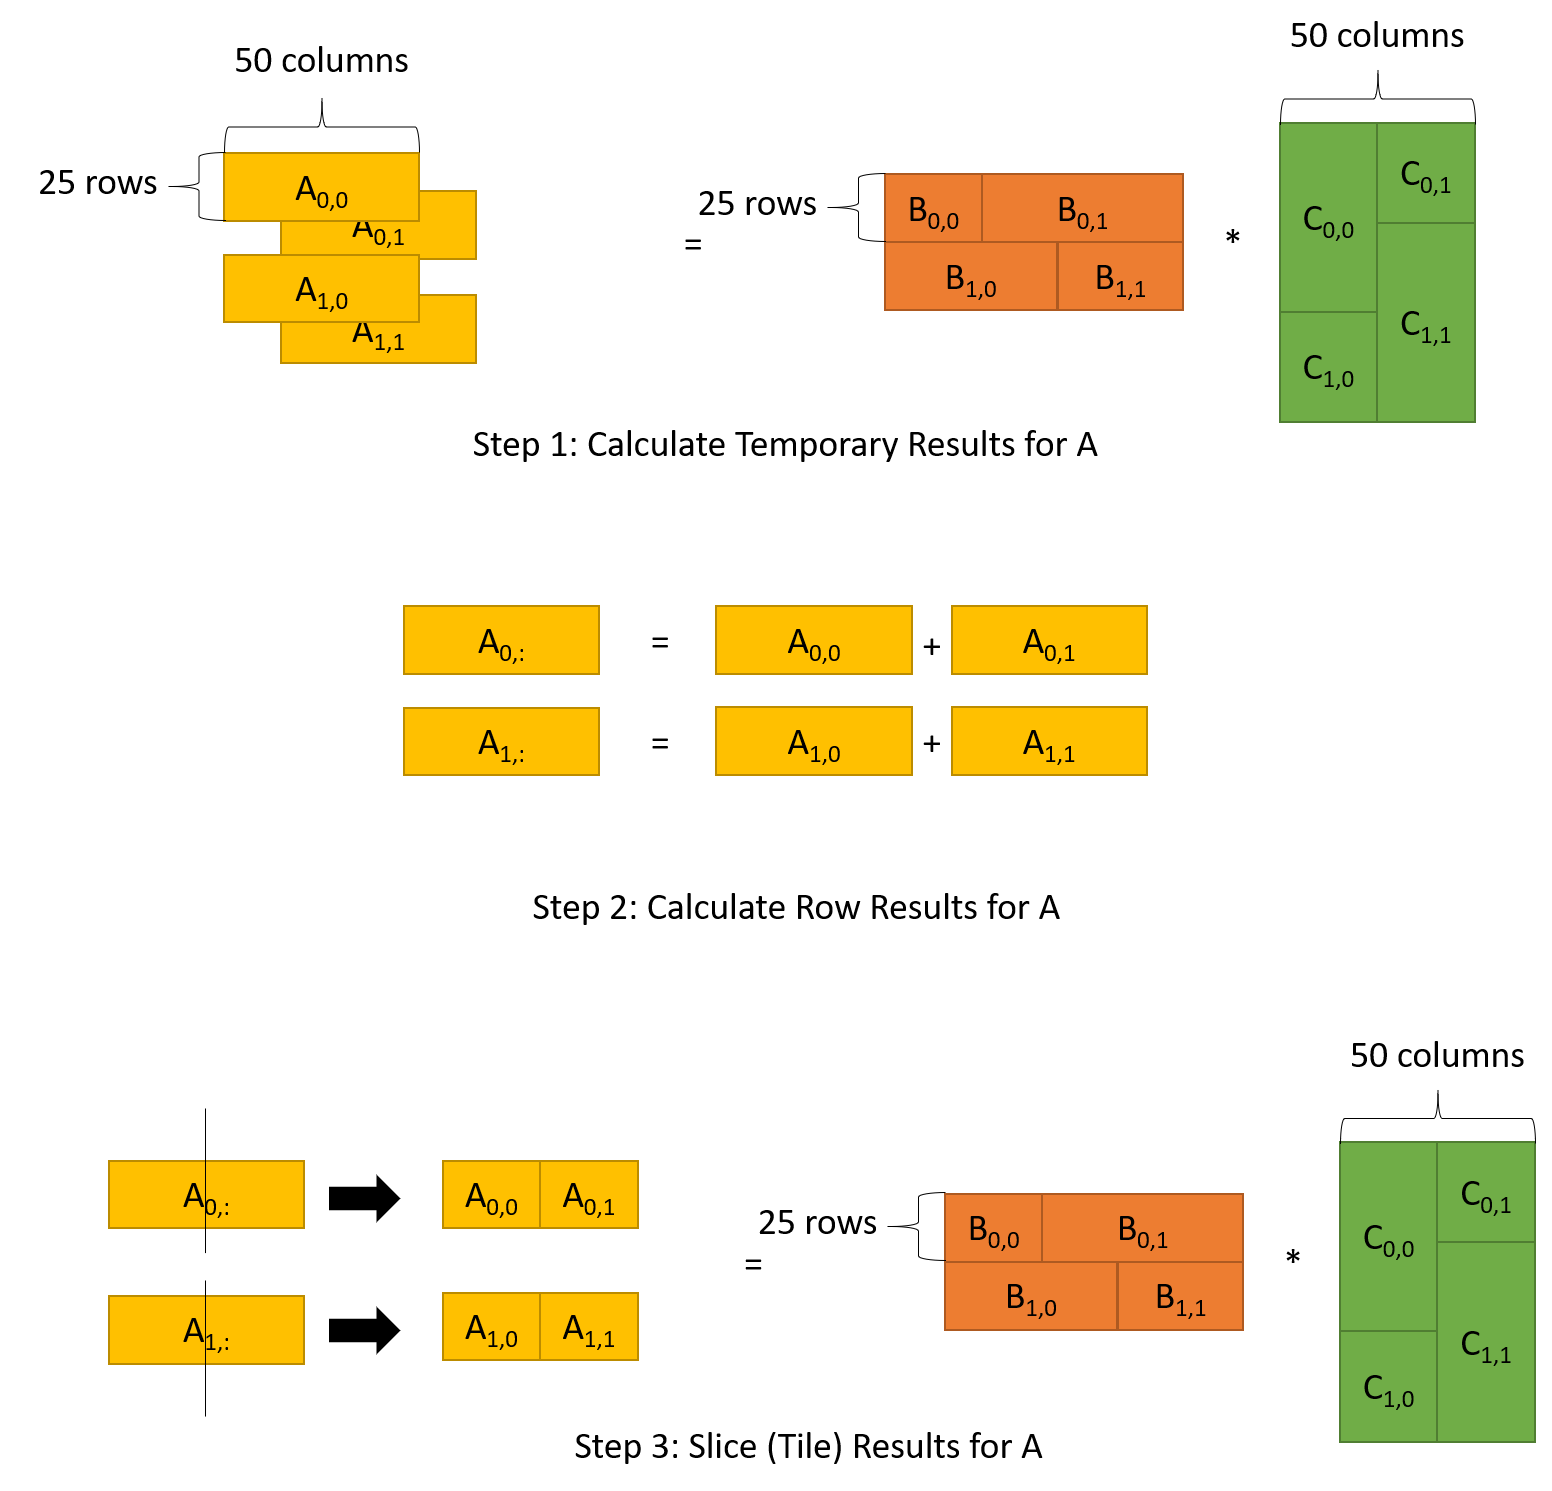
\includegraphics[width=0.66\linewidth]{figures/intermediate_result_sum.png}
		\caption{Calculating Final Tiled Result}
	\end{figure}
\end{frame}

\begin{frame}{dot\_d Example: $A = B \cdot C$ }
	\begin{figure}	
		\centering
		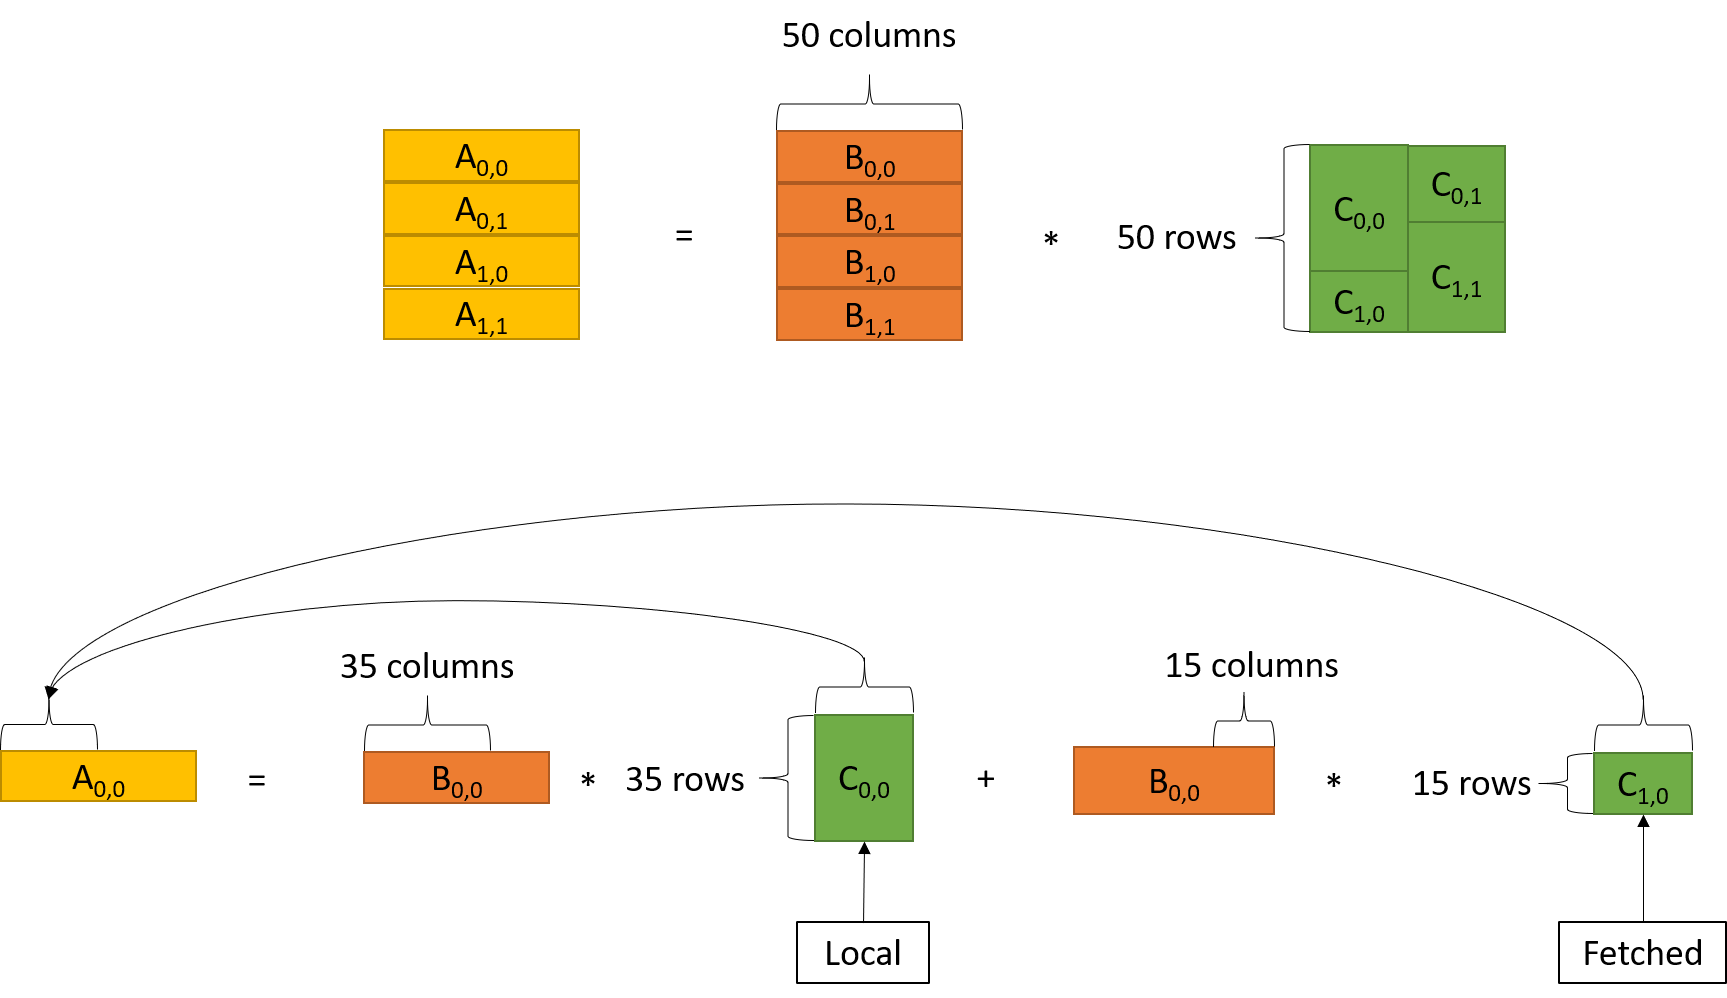
\includegraphics[width=0.66\linewidth]{figures/row_major_lhs_dot_d.png}
		\caption{Row Major LHS}
	\end{figure}
\end{frame}

\begin{frame}{Cannon's Algorithm}
	\begin{outline}
		\1 Space efficient matrix multiplication algorithm
		\1 Moves both input matrix tiles at every step
			\2 $\sqrt{P}$ number of iterations (on $P$ processors)
		\1 End result does not require row-aggregation
	\end{outline}
\end{frame}

\begin{frame}{Cannon Example: $A = B \cdot C$}
	\begin{figure}	
		\centering
		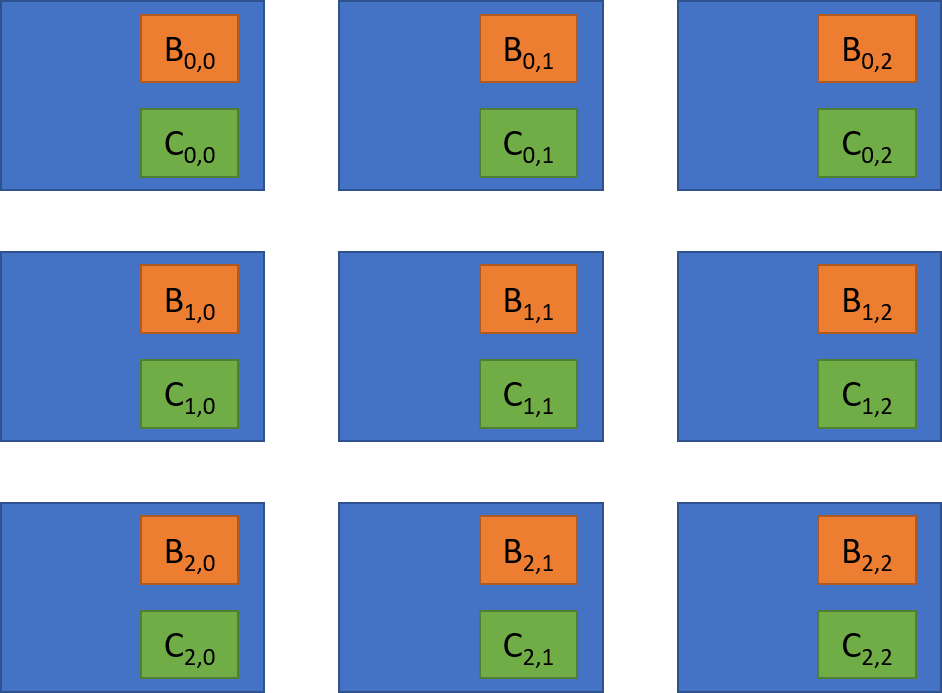
\includegraphics[width=0.72\linewidth]{figures/cannon_zeroth_iteration.png}
		\caption{Alignment}
	\end{figure}
\end{frame}

\begin{frame}{Cannon Example: $A = B \cdot C$}
	\begin{figure}	
		\centering
		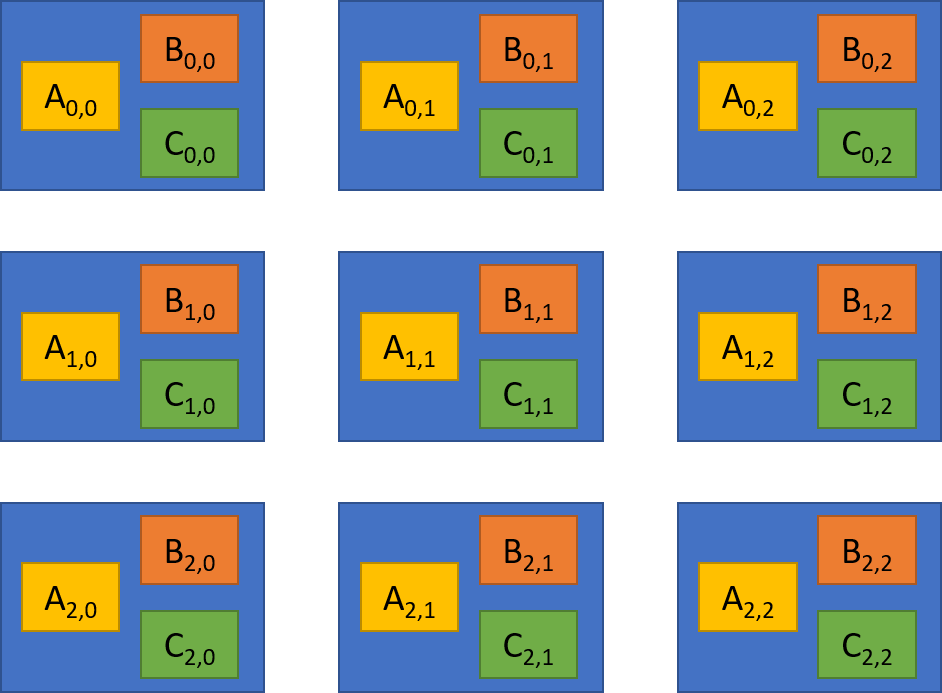
\includegraphics[width=0.72\linewidth]{figures/cannon_start.png}
		\caption{Multiply Local Values}
	\end{figure}
\end{frame}

\begin{frame}{Cannon Example: $A = B \cdot C$}
	\begin{figure}	
		\centering
		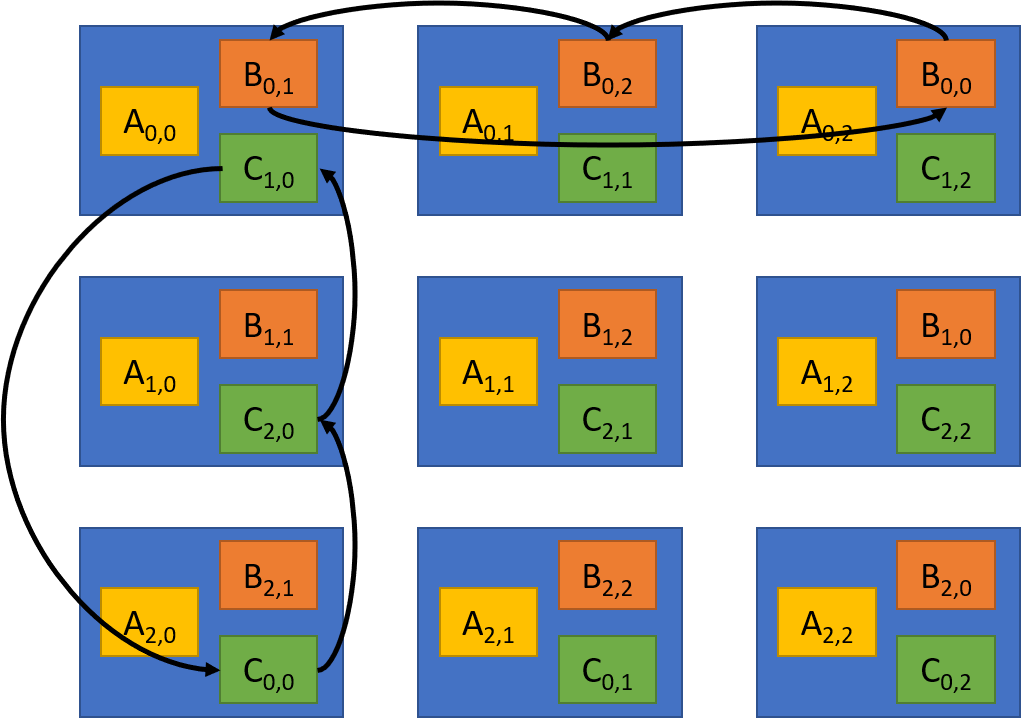
\includegraphics[width=0.72\linewidth]{figures/cannon_first_iteration.png}
		\caption{Shift Data \& multiply}
	\end{figure}
\end{frame}

\begin{frame}{Cannon Example: $A = B \cdot C$}
\begin{figure}	
	\centering
	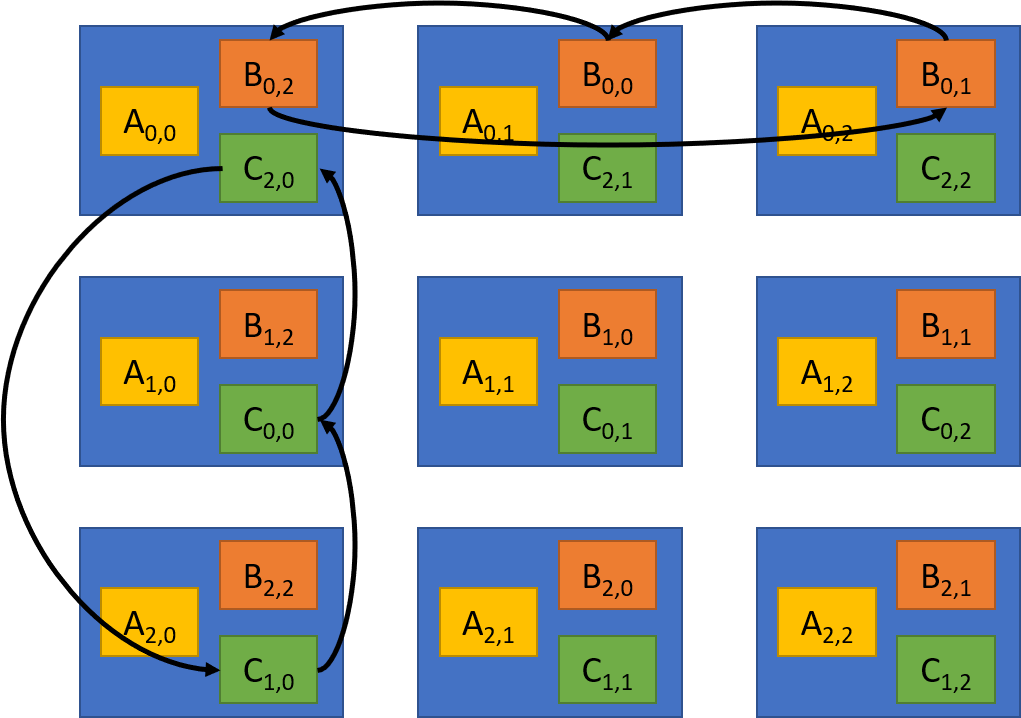
\includegraphics[width=0.72\linewidth]{figures/cannon_second_iteration.png}
	\caption{Shift Data \& multiply}
\end{figure}
\end{frame}

\begin{frame}{Futurizing Cannon's Algorithm}
	\begin{outline}
		\1 No permanent data moving
			\2 Pulling instead
			\2 Doubles memory cost
		\1 Allows pulling to be done one cycle ahead
			\2 Computation runs while data is being fetched
	\end{outline}
\end{frame}


\section{Results \& Future Work}

\begin{frame}{Preliminary Results}
	\begin{columns}
		\column{0.4\linewidth}
		\begin{outline}
			\1 Both distributed algorithms outperformed the pure serial version
			\1 Cannon performed substantially better than dot\_d
		\end{outline}

		\column{0.75\linewidth}
		\centering
		\begin{tabular}{|c|c|c|c|} \hline
			Matrix Size	& dot\_d & cannon & dot (serial)\\ \hline
			500	 & 5351.08 &	3131.345 &	8538.37\\ \hline
			1000 & 36946.15 & 25889.2	& 67425.2\\ \hline
			2000 & 282916.5	& 170091.5	& 539491\\ \hline		
		\end{tabular}
	\end{columns}
\end{frame}

\begin{frame}{Speedup}
	\begin{figure}	
		\centering
		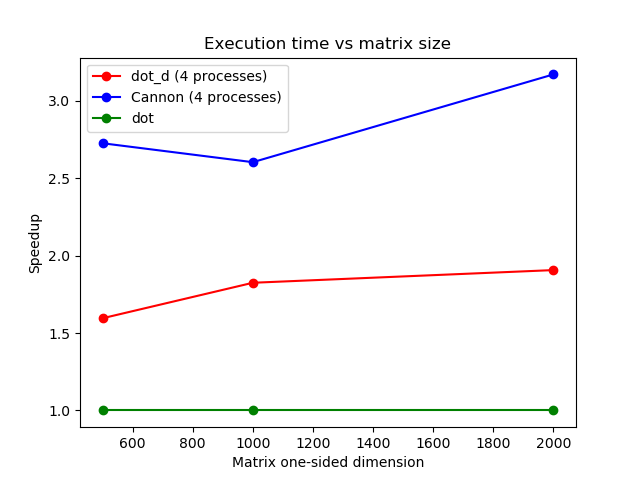
\includegraphics[width=0.82\linewidth]{figures/speed_up_plot.png}
		\caption{Speedup Plot}
	\end{figure}
\end{frame}

\begin{frame}{Contributions of this work}
	\begin{outline}
		\1 Explored performance and implementation differences between two different matrix multiplication algorithms
		\1 Learned more about how tiling structure impacts performance
			\2 In how it is derived from the algorithm
			\2 In how we might choose algorithms for their tiling benefits or constraints
		\1 Learned more about our requirements for distributed primitives in Phylanx going forward
		\1 Highlighted known deficiencies in HPX that, if resolved, would improve distributed functionality
				
	\end{outline}
\end{frame}

\begin{frame}{Future Work}
	\begin{outline}
		\1 Confirm results in a cluster environment
		\1 Tiling testing
		\1 Tiling optimizer
	\end{outline}
\end{frame}

\begin{frame}[standout]
	Questions?
\end{frame}

\begin{frame}{Complexity}
	\begin{outline}
		\1 In an operation, $A = B \cdot C, B \in M_{NxL}, C \in M_{LxM}$, with $B, C$ containing doubles (8 bytes)
		\1 Cannon’s algorithm always transfers $8*(\sqrt{P}*(N*L/P)+\sqrt{P}*(L*M/P))$ bytes of data at a speed of $\alpha$ bytes/sec, with latency $\beta$, meaning it takes $\sqrt{P}*\beta$ time in latency, due to the futurization, with a total maximum memory footprint of $(N*M)+2*(N*L)+2*(L*M)$.
		\1 dot\_d transfers up to $8*P*(P-1)*(L*M)$ bytes of data in the main multiplication step, and up to $8*N*log(L)*M$ bytes in the row-aggregation step, with total latency $P*(P-1)*\beta+N*log(L)*\beta$ in the worst case. The memory footprint in the worst case is $P*(N*M)+(N*L)+2*(L*M)$
		
	\end{outline}
\end{frame}

\end{document}
